\documentclass[10pt]{article}          % the type of document and font size (default 10pt)
\usepackage[a4paper, tmargin=1.0in, bmargin=1.0in, lmargin=0.5in, rmargin=0.5in]{geometry}   
                                      % sets all margins to 1in, can be changed
\usepackage{moreverb}                 % for verbatimtabinput -- LaTeX environment
\usepackage{url}                      % for \url{} command
\usepackage{amssymb}                  % for many mathematical symbols
\usepackage[pdftex]{lscape}           % for landscaped tables
\usepackage{longtable}                % for tables that break over multiple pages
\usepackage[utf8]{inputenc}           % UTF8 characters
\usepackage[T1]{fontenc}
\usepackage{textcomp}
\usepackage[english]{babel}
\usepackage{float}                    % Position of figure, table
\usepackage{enumitem}                 % Alphabet list
\usepackage{makecell}                 % Customize cells in a table
\usepackage{amsmath}
\usepackage{amsfonts}
\usepackage{amssymb}
\usepackage{mathtools}
\usepackage{mathrsfs}
\usepackage{graphicx}
\usepackage{babel,blindtext}
\usepackage{ulem}
\usepackage{tabularx}
\usepackage[table]{xcolor}
\graphicspath{ {../output/} }
\DeclarePairedDelimiter{\ceil}{\lceil}{\rceil}
\renewcommand{\baselinestretch}{1.5}
\title{COCS 6323: Statistical Methods in Research \\ Group Project} % to specify title
\author{Group 2 \\
        Department of Computer Science\\
        University of Houston}         % to specify author(s)
\usepackage{Sweave}
\begin{document}                      % document begins here
\Sconcordance{concordance:ProjectReport.tex:ProjectReport.Rnw:%
1 31 1 1 0 13 1}
\Sconcordance{concordance:ProjectReport.tex:././sections/contribution2.Rnw:ofs 46:%
1 11 1}
\Sconcordance{concordance:ProjectReport.tex:ProjectReport.Rnw:ofs 58:%
47 2 1}
\Sconcordance{concordance:ProjectReport.tex:././sections/section4.Rnw:ofs 61:%
1 9 1}
\Sconcordance{concordance:ProjectReport.tex:ProjectReport.Rnw:ofs 71:%
51 2 1}
\Sconcordance{concordance:ProjectReport.tex:././sections/sectionT2.Rnw:ofs 74:%
1 32 1}
\Sconcordance{concordance:ProjectReport.tex:ProjectReport.Rnw:ofs 107:%
55 2 1}
\Sconcordance{concordance:ProjectReport.tex:././sections/sectionT3.Rnw:ofs 110:%
1 65 1}
\Sconcordance{concordance:ProjectReport.tex:ProjectReport.Rnw:ofs 176:%
59 4 1}


\setkeys{Gin}{width=1.0\textwidth}

\maketitle              % makes the title

\newpage
\tableofcontents        % inserts TOC (section, sub-section, etc numbers and titles)
\listoftables           % inserts LOT (numbers and captions)
\listoffigures          % inserts LOF (numbers and captions)

\newpage
\section{Contribution}
% !Rnw root = ../ProjectReport.Rnw
\begin{table}[h]
\begin{tabular}{|p{4cm}|p{13cm}|}
\hline
\textbf{Member} & \textbf{Contribution} \\ \hline
Bradley Macdonald & Analyze regression models of Figure 4\\ \hline
Tung Huynh & Preprocess Data, create and analyze regression models of Table S2, Table S3\\ \hline
Yifan Zhang & Preprocess Data, and draw plot of Figure 4 \\ \hline
\end{tabular}
\caption{Contribution of group members of the second milestone}
\label{tbl:contribution}
\end{table}

\newpage
\section{Figure 5}
% !Rnw root = ../ProjectReport.Rnw
\begin{figure}[!htb]
  \minipage{0.5\textwidth}
    \textbf{A}\\
    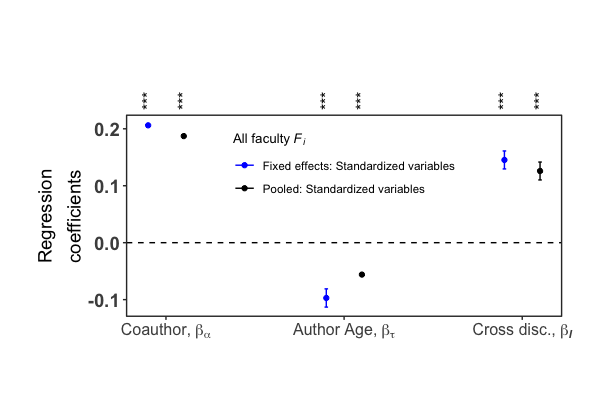
\includegraphics[width=9.3cm, height=7cm]{5A.png}
  \endminipage\hfill
  \minipage{0.5\textwidth}%
    \textbf{B}\\
    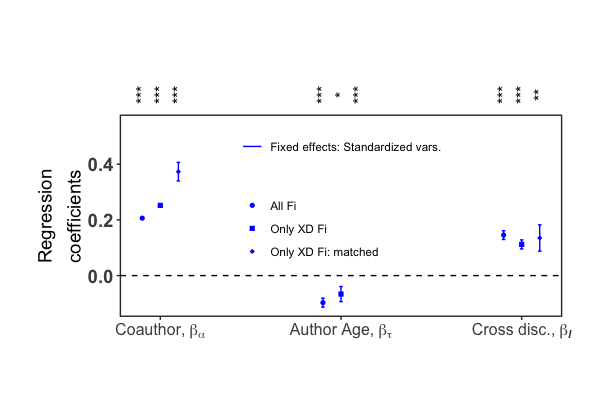
\includegraphics[width=9.3cm, height=7cm]{5B.png}
  \endminipage\hfill
  \minipage{0.5\textwidth}
    \textbf{C}\\
    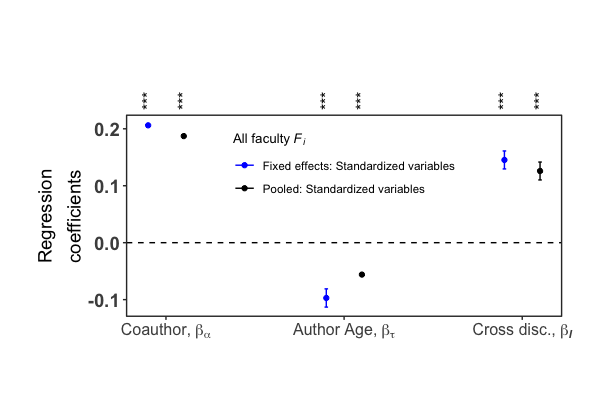
\includegraphics[width=9.3cm, height=7cm]{5A.png}
  \endminipage\hfill
  \minipage{0.5\textwidth}%
    \textbf{D}\\
    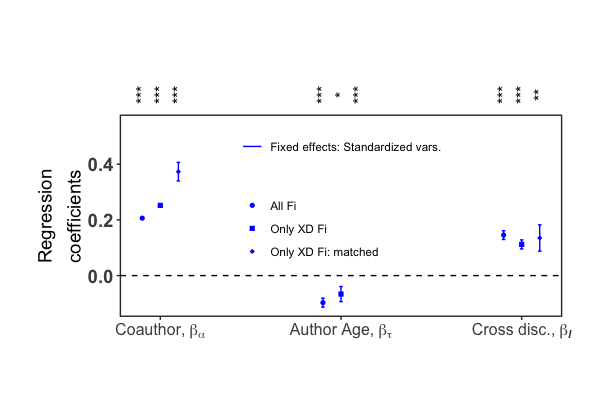
\includegraphics[width=9.3cm, height=7cm]{5B.png}
  \endminipage
  \caption{Career panel regression model}
  \label{fig:2A}
\end{figure}


\newpage
\section{Supplementary Table S4}
% !Rnw root = ../ProjectReport.Rnw
\begin{table}[H]
\begin{tabular}{m{5cm} m{3.0cm} m{3cm} m{2.5cm} m{2.7cm}}
\hline
\hline
& \textbf{No Fixed Effects} & \textbf{No Fixed Effects [Standardized]} & \textbf{Fixed Effects} & \textbf{Fixed Effects [Standardized]} \\ \hline
\multicolumn{5}{l}{\textbf{Publication characteristics}} \\
\rowcolor{lightgray}
{\# of author, $\beta_\alpha$} & 0.2836*** & 0.1872*** & 0.312*** & 0.2061*** \\
                             & (0.0025) & (0.0016) & (0.00262) & (0.00173) \\
\rowcolor{lightgray}
{Career age, $\beta_\tau$} & -0.00547*** & -0.0560*** & -0.00949*** & -0.0971*** \\
                         & (0.0002) & (0.0018) & (0.00156) & (0.01601) \\
\rowcolor{lightgray}
{Cross-disciplinary indicator, $\beta_I$} & 0.1259*** & 0.1259*** & 0.1453*** & 0.1453*** \\
                                        & (0.0157) & (0.0157) & (0.01578) & (0.01578) \\ \hline
\multicolumn{5}{l}{\textbf{Network characteristics}} \\
\rowcolor{lightgray}
{Author centrality, $\beta_\zeta$} & 0.0440*** & 0.0284*** & X & X \\
                             & (0.0029) & (0.0018) &  &  \\
\rowcolor{lightgray}
{Bridge ratio, $\beta_\lambda$} & 0.3338*** & 0.1210*** & X & X \\
                             & (0.0055) & (0.0020) &  &  \\
\rowcolor{lightgray}
{Discipline ($F$) dummy}     & 0.00790* & 0.0079* & X & X \\
                             & (0.0033) & (0.0033) & &  \\
\rowcolor{lightgray}
{Constant}                 & 0.4586*** & 0.1638* & -0.2932*** & -0.0669** \\
                         & (0.0761) & (0.0728) & (0.0456) & (0.0176) \\
\rowcolor{lightgray}
{Year dummy}            & Y & Y & Y & Y \\ \hline
\rowcolor{lightgray}
{n}                      & 413,565 & 413,565 & 413,565 & 413,565 \\
\rowcolor{lightgray}
{adj. $R^2$}             & 0.055 & 0.055 & 0.036 & 0.036 \\ \hline \hline
\multicolumn{5}{l}{\footnotesize{Standard errors in parentheses below estimate * p $\leq$ 0.05, ** p $\leq$ 0.01, *** p $\leq$ 0.0001}}

\end{tabular}
\caption{Career data set: Panel model on all falcuty}
\label{tbl:sT5}
\end{table}

\newpage
\section{Supplementary Table S5}
% !Rnw root = ../ProjectReport.Rnw
\begin{table}[H]
\begin{tabular}{m{5cm} m{3.0cm} m{3cm} m{2.5cm} m{2.7cm}}
\hline
\hline
& \textbf{No Fixed Effects} & \textbf{No Fixed Effects [Standardized]} & \textbf{Fixed Effects} & \textbf{Fixed Effects [Standardized]} \\ \hline
\multicolumn{5}{l}{\textbf{Publication characteristics}} \\
\rowcolor{lightgray}
{\# of author, $\beta_\alpha$} & 0.329***  & 0.236*** & 0.351*** & 0.252*** \\
                             & (0.0037) & (0.0027) & (0.00392) & (0.00282) \\
\rowcolor{lightgray}
{Career age, $\beta_\tau$} & -0.00499*** & -0.0536*** & -0.00617* & -0.0663* \\
                         & (0.0003) & (0.0030) & (0.00253) & (0.0271) \\
\rowcolor{lightgray}
{Cross-disciplinary indicator, $\beta_I$} & 0.1095*** & 0.1095*** &  0.112*** & 0.112*** \\
                                        & (0.0165) & (0.0165) & (0.0162) & (0.0162) \\ \hline
\multicolumn{5}{l}{\textbf{Network characteristics}} \\
\rowcolor{lightgray}
{Author centrality, $\beta_\zeta$} & 0.0526*** & 0.0333*** & X & X \\
                             & (0.0046) & (0.0029) &  &  \\
\rowcolor{lightgray}
{Bridge ratio, $\beta_\lambda$} & 0.3192*** & 0.1116*** & X & X \\
                             & (0.0092) & (0.0032) & & \\
\rowcolor{lightgray}
{Discipline ($F$) dummy}     & -0.0383*** & -0.0383*** & X & X \\
                             & (0.0052) & (0.0052) & & \\
\rowcolor{lightgray}
{Constant}                 & 0.2113 & -0.0287 & -0.408*** & -0.0370* \\
                         & (0.1236) & (0.1187) & (0.0778) & (0.0285) \\
\rowcolor{lightgray}
{Year dummy}            & Y & Y & Y & Y \\ \hline
\rowcolor{lightgray}
{n}                      & 166,621 & 166,621 & 166,621 & 166,621 \\
\rowcolor{lightgray}
{adj. $R^2$}             & 0.067 & 0.067 & 0.049 & 0.049 \\ \hline \hline
\multicolumn{5}{l}{\footnotesize{Standard errors in parentheses below estimate * p $\leq$ 0.05, ** p $\leq$ 0.01, *** p $\leq$ 0.0001}}

\end{tabular}
\caption{Career data set: Panel model on all $XD_F$ falcuty}
\label{tbl:sT5}
\end{table}

\newpage
\section{Supplementary Table S6}
% !Rnw root = ../ProjectReport.Rnw
\begin{table}[H]
\begin{tabular}{m{5cm} m{3.0cm} m{3cm} m{2.5cm} m{2.7cm}}
\hline
\hline
& \textbf{No Fixed Effects} & \textbf{No Fixed Effects [Standardized]} & \textbf{Fixed Effects} & \textbf{Fixed Effects [Standardized]} \\ \hline
\multicolumn{5}{l}{\textbf{Publication characteristics}} \\
\rowcolor{lightgray}
{\# of author, $\beta_\alpha$} & 0.329***  & 0.236*** & 0.351*** & 0.252*** \\
                             & (0.0037) & (0.0027) & (0.00392) & (0.00282) \\
\rowcolor{lightgray}
{Career age, $\beta_\tau$} & -0.00499*** & -0.0536*** & -0.00617* & -0.0663* \\
                         & (0.0003) & (0.0030) & (0.00253) & (0.0271) \\
\rowcolor{lightgray}
{Cross-disciplinary indicator, $\beta_I$} & 0.1095*** & 0.1095*** &  0.112*** & 0.112*** \\
                                        & (0.0165) & (0.0165) & (0.0162) & (0.0162) \\ \hline
\multicolumn{5}{l}{\textbf{Network characteristics}} \\
\rowcolor{lightgray}
{Author centrality, $\beta_\zeta$} & 0.0526*** & 0.0333*** & X & X \\
                             & (0.0046) & (0.0029) &  &  \\
\rowcolor{lightgray}
{Bridge ratio, $\beta_\lambda$} & 0.3192*** & 0.1116*** & X & X \\
                             & (0.0092) & (0.0032) & & \\
\rowcolor{lightgray}
{Discipline ($F$) dummy}     & -0.0383*** & -0.0383*** & X & X \\
                             & (0.0052) & (0.0052) & & \\
\rowcolor{lightgray}
{Constant}                 & 0.2113 & -0.0287 & -0.408*** & -0.0370* \\
                         & (0.1236) & (0.1187) & (0.0778) & (0.0285) \\
\rowcolor{lightgray}
{Year dummy}            & Y & Y & Y & Y \\ \hline
\rowcolor{lightgray}
{n}                      & 166,621 & 166,621 & 166,621 & 166,621 \\
\rowcolor{lightgray}
{adj. $R^2$}             & 0.067 & 0.067 & 0.049 & 0.049 \\ \hline \hline
\multicolumn{5}{l}{\footnotesize{Standard errors in parentheses below estimate * p $\leq$ 0.05, ** p $\leq$ 0.01, *** p $\leq$ 0.0001}}

\end{tabular}
\caption{Career data set: Panel model on all $XD_F$ falcuty: matching}
\label{tbl:sT5}
\end{table}

\bigskip   % leave some empty space (optional)

\end{document}

